
\section{Results: Differences in Spring Chemistry and Residence Time}

\subsection{Traverse 1}

\begin{figure}[h]
    \centering
        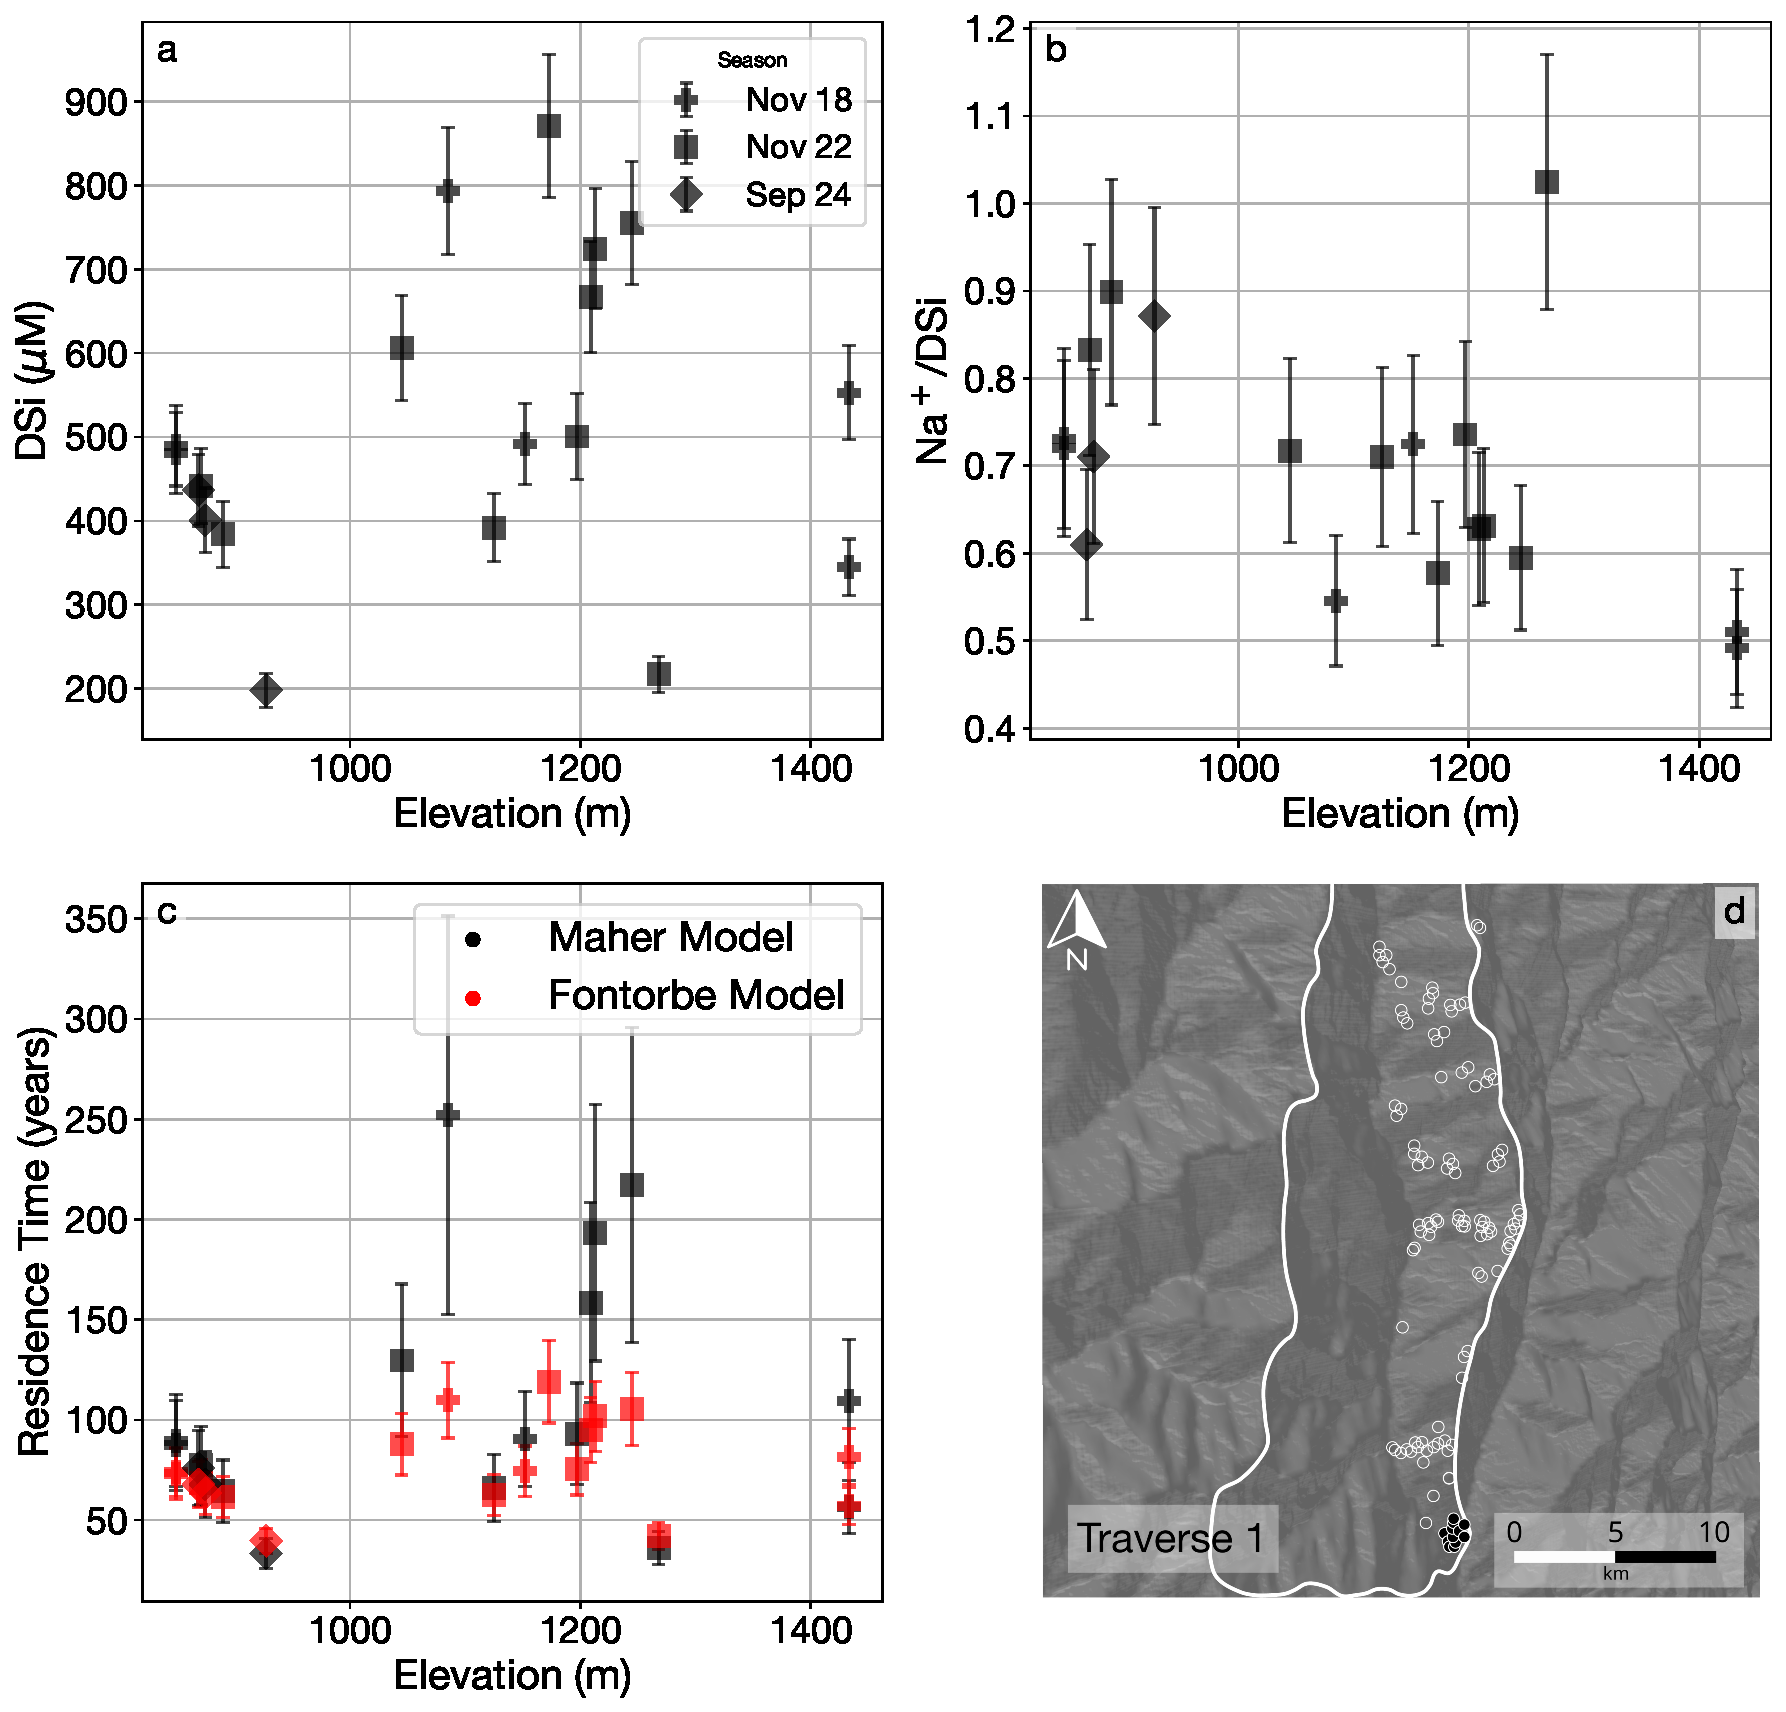
\includegraphics[width=\textwidth]{Traverse_1_summary.pdf}
    \caption{Traverse 1 - Variations in Spatial Chemistry}
    \label{fig:spatial_changes_spring1}
\end{figure}

\FloatBarrier

Concentration of dissolved silicon (DSi) in the springs sampled in Traverse 1 is at a maximum for the whole catchment. There is no clear trend of increasing DSi concentration with decreasing elevation, but Na/Si does increase with the same x-axis. The Fontorbe model predicts a peak of $\approx$ 100 years, while the Maher model predicts a much higher residence time of $\approx$ 600 years. Strontium isotopes are also at a maximum in this traverse, but there is no resolvable mixing trend; strontium isotope ratios used alongside strontium concentrations can be used to determine mixing between different endmembers (Faure, 1986; See Appendix).



\newpage

\subsection{Traverse 2}

\begin{figure}[h]
    \centering
        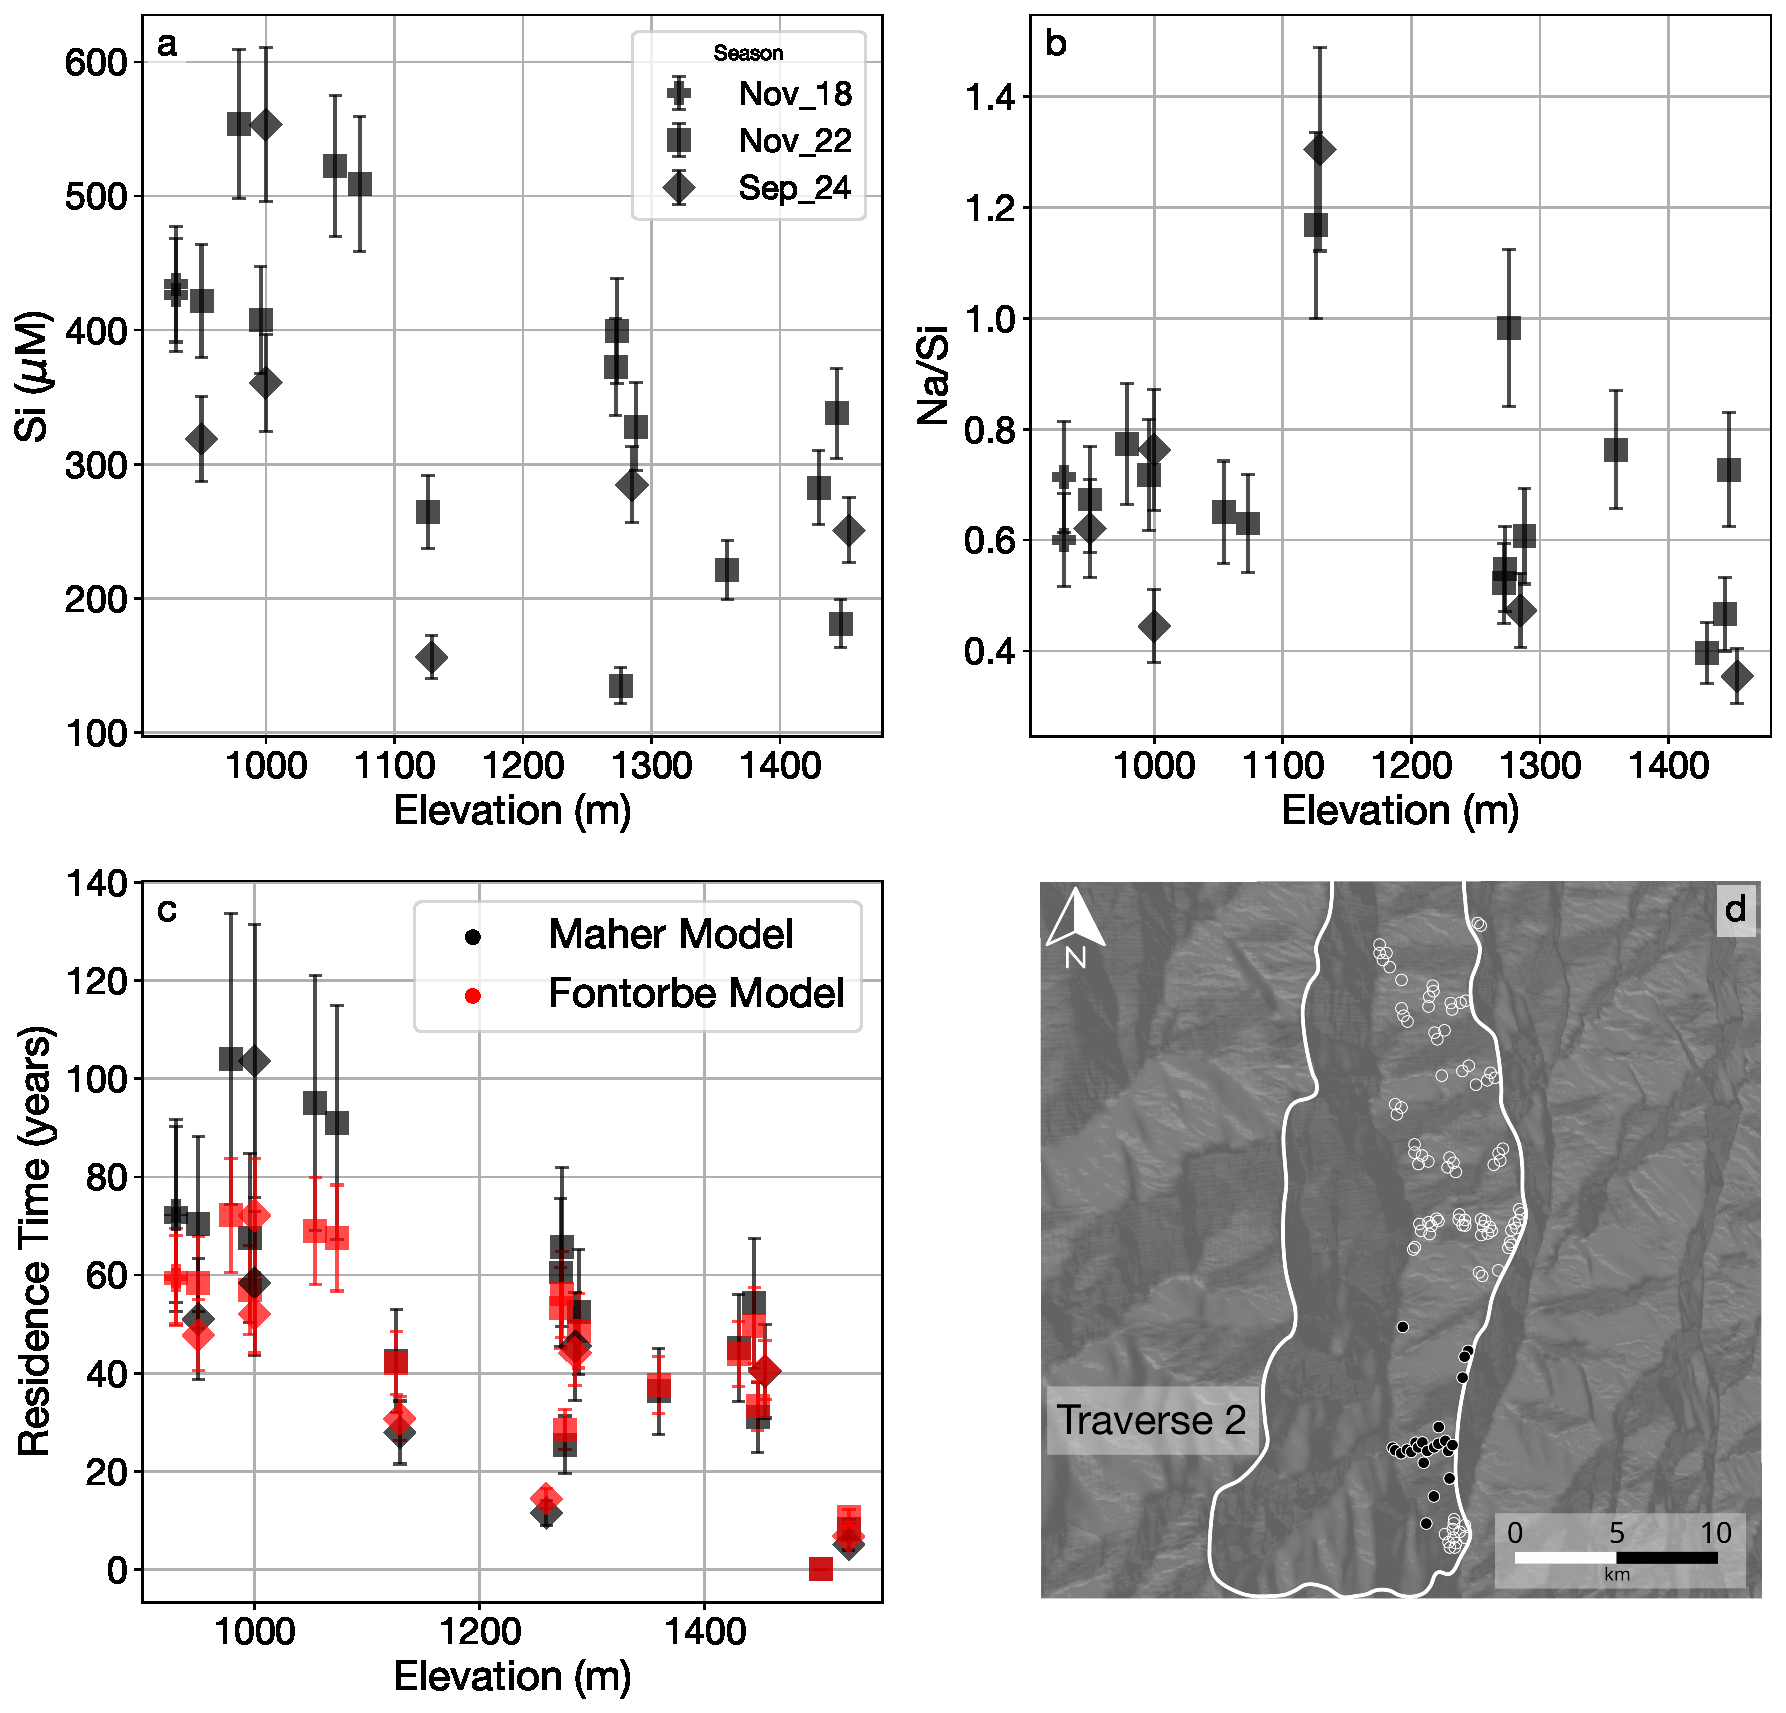
\includegraphics[width=\textwidth]{Traverse_2_summary.pdf}
    \caption{Traverse 2 - Variations in Spatial Chemistry}
    \label{fig:spatial_changes_spring2}
\end{figure}

\FloatBarrier

Dissolved silicon concentration shows a clear increase in concentration with decreasing elevation. There is no resolvable trend with Na/Si and elevation, nor with different seasons when it was collected. Residence times are generally lower than those in Traverse 1, but the Maher model is still higher at lower elevations, predicting a maximum of $\approx$ 100 years. The Fontorbe model predicts generally older times than the Maher model at higher elevations, and lower times at lower elevations. Strontium isotopes are in the same range as those in Traverse 1. Here, a mixing trend is resolvable given by a straight line with a R$^2$ of (?).


% The lack of trend in Na/Si against elevation space, coupled with the consistent increase in DSi suggests little reprecipitation is occuring in this traverse. The lower residence times compared to Traverse 1 are consistent with shorter flow paths at higher elevation, considering rainfall which acts as an input to the system is delivered mostly to the top quarter of the catchment, which Traverse 2 is not in. Mixing trends in strontium isotopes suggest a varying lithology that the springs travel through.



\newpage

\subsection{Traverse 3}

\begin{figure}[h]
    \centering
        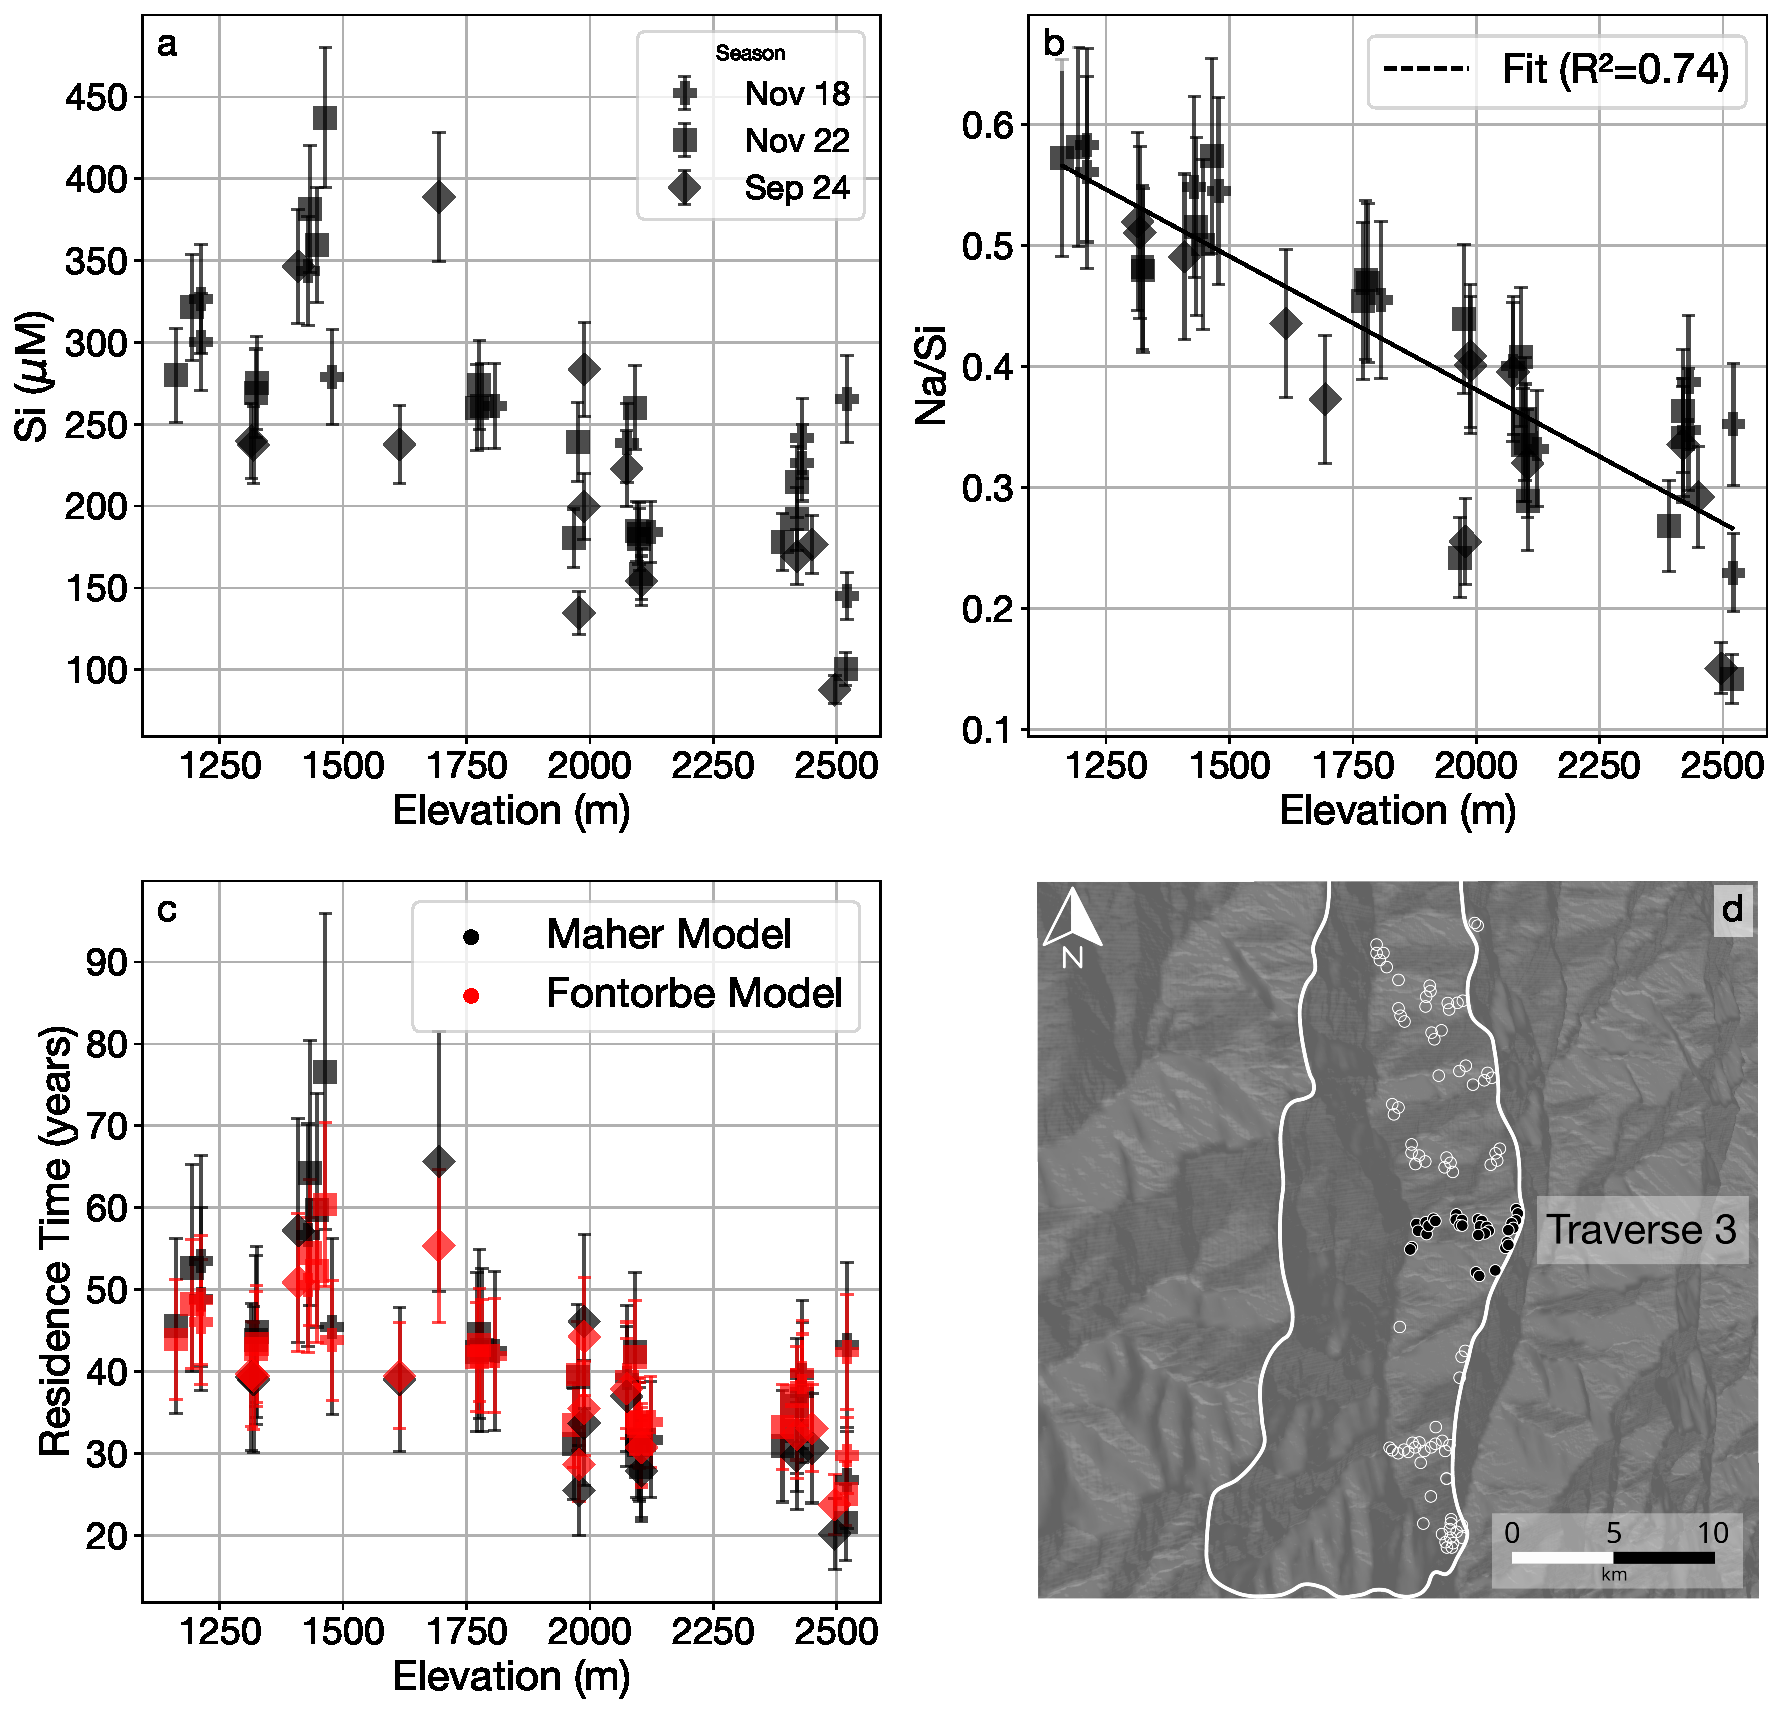
\includegraphics[width=\textwidth]{Traverse_3_summary.pdf}
    \caption{Traverse 3 - Variations in Spatial Chemistry}
    \label{fig:spatial_changes_spring3}
\end{figure}

\FloatBarrier

Dissolved silicon concentration increases with decreasing elevation in Traverse 3. There is a potential dip at the lowermost elevation sampled. Na/Si showcases a consistent increase with decreasing elevation, and this trend carries through between different seasons. Residence times predicted increase as elevation decreases, peaking at $\approx$ 50 years for the Maher model. At the very end of the flow path, however, both the Maher and Fontorbe model predict $\approx$ 25 years. Strontium isotopes do not showcase a clear mixing trend, and the radiogenic strontium isotope values are lower than those found in Traverse 1 and 2. 


\newpage

\subsection{Traverse 4}

\begin{figure}[h]
    \centering
        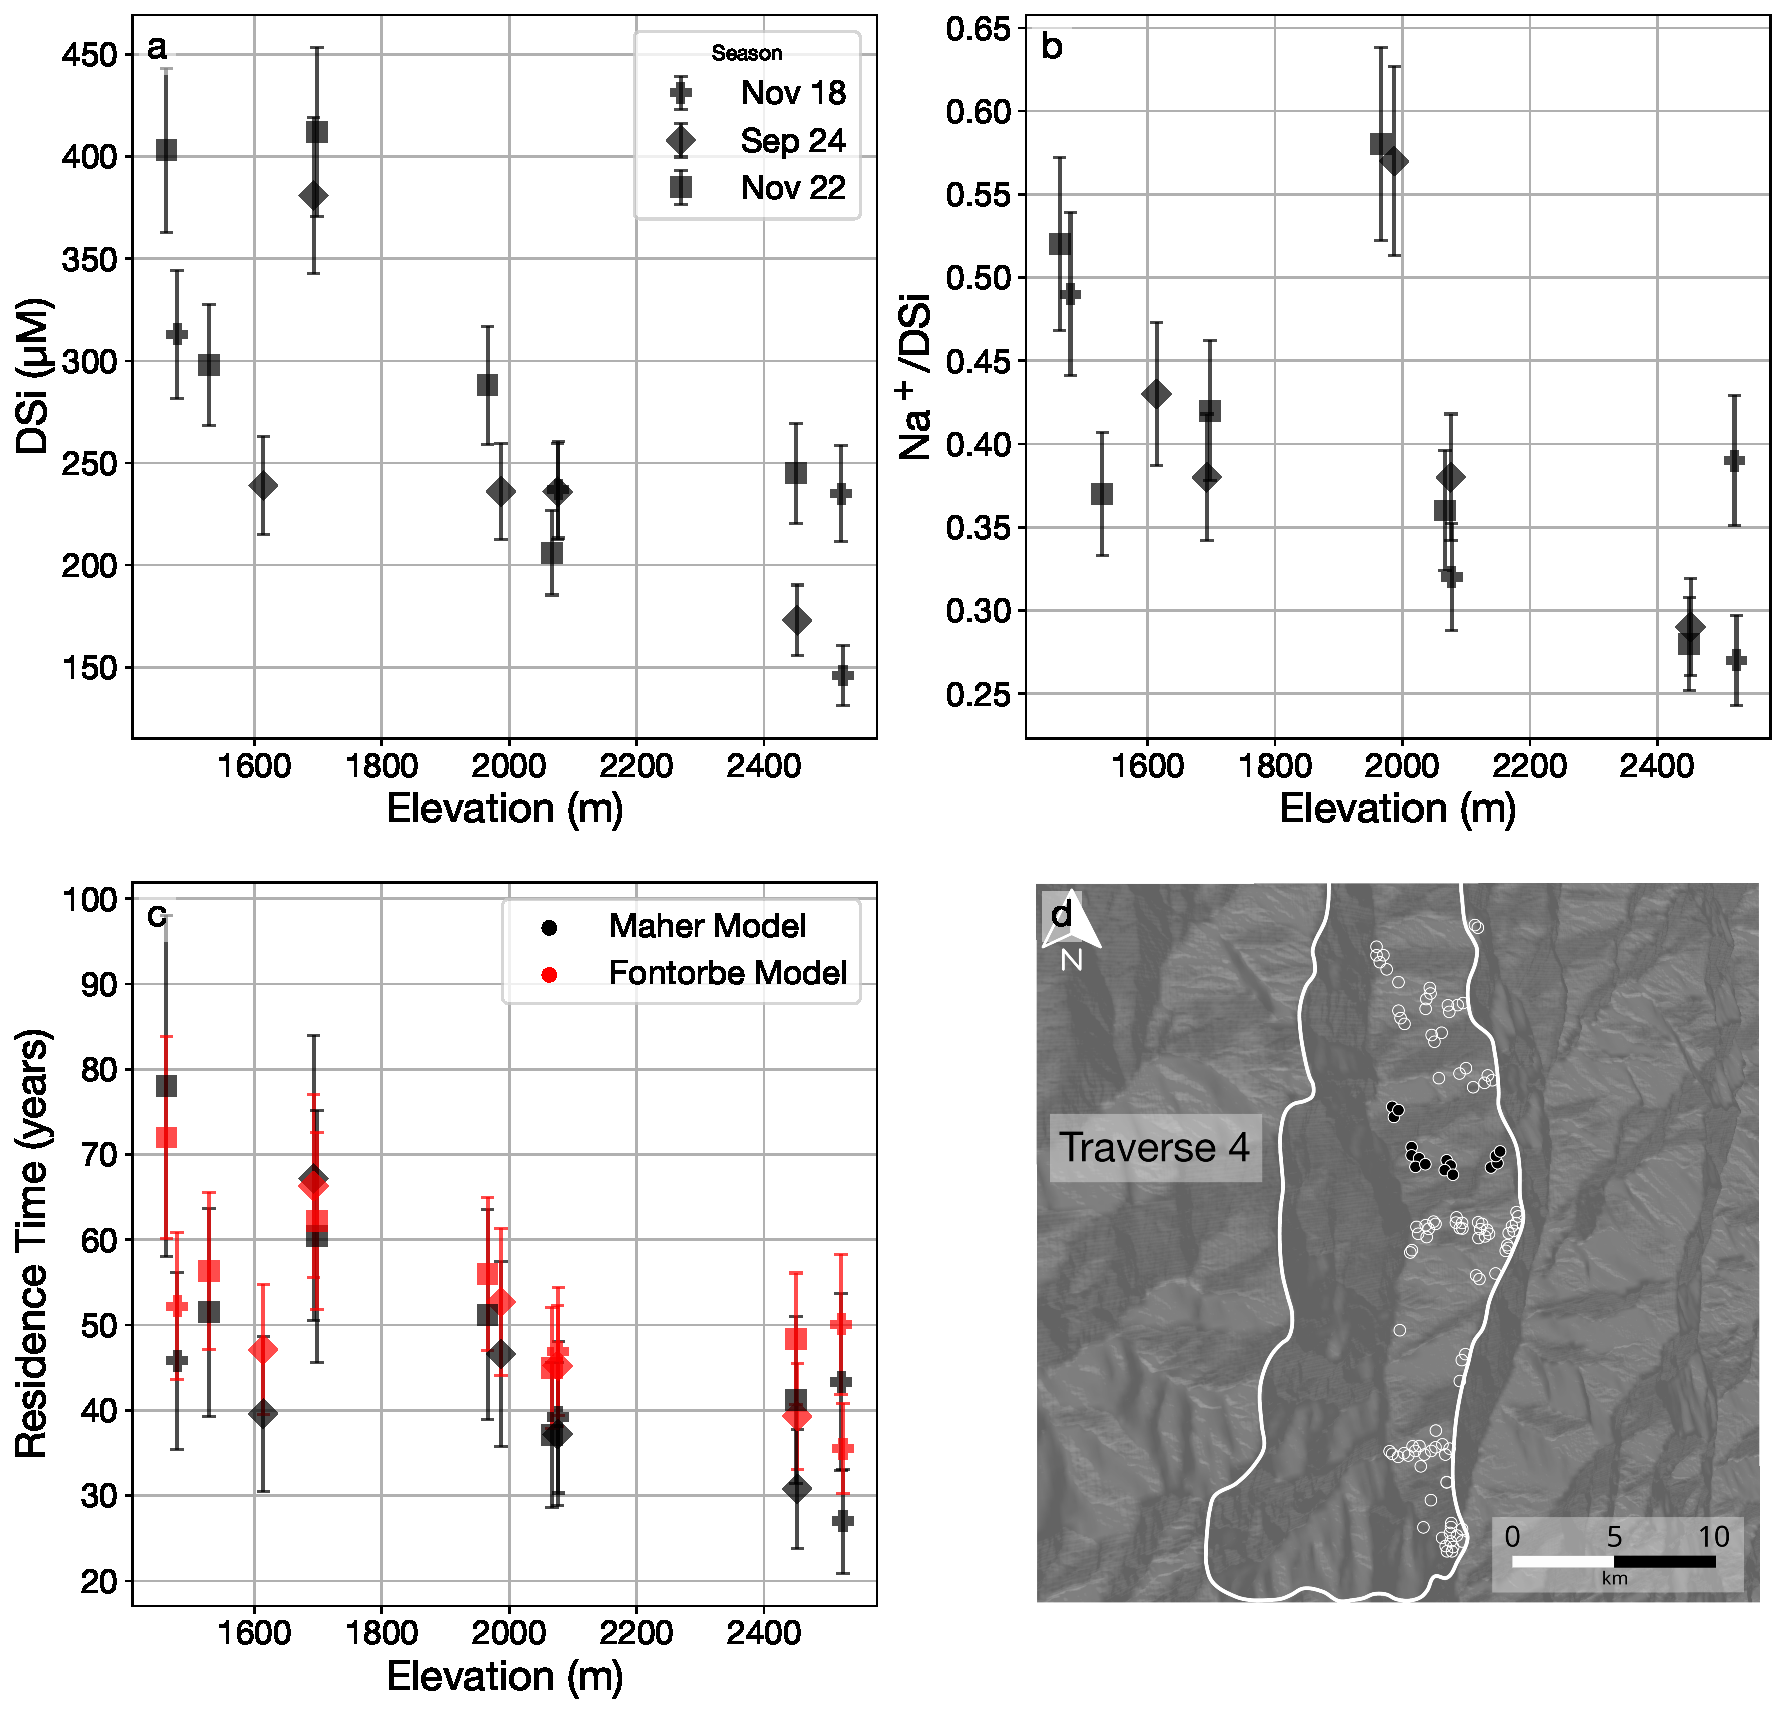
\includegraphics[width=\textwidth]{Traverse_4_summary.pdf}
    \caption{Traverse 4 - Variations in Spatial Chemistry}
    \label{fig:spatial_changes_spring4}
\end{figure}

\FloatBarrier

Traverse 4 is undersampled compared to the other traverses. Given the small sample set, any apparent trend is less to be reflective of the true chemistry. Nevertheless, DSi increases with decreasing elevation as seen in some of the previous traverses. There is no discernable trend with Na/Si. Residence times also increase with decreasing elevation, with the Maher model predicting younger times at the highest elevations, and older times at the lowest elevations. The highest residence times predicted are $\approx$ 35 years. Strontium isotopes do not show a clear mixing trend, but the minimum signature is lower than that of Traverse 3.

\newpage

\subsection{Traverse 5}

\begin{figure}[h]
    \centering
        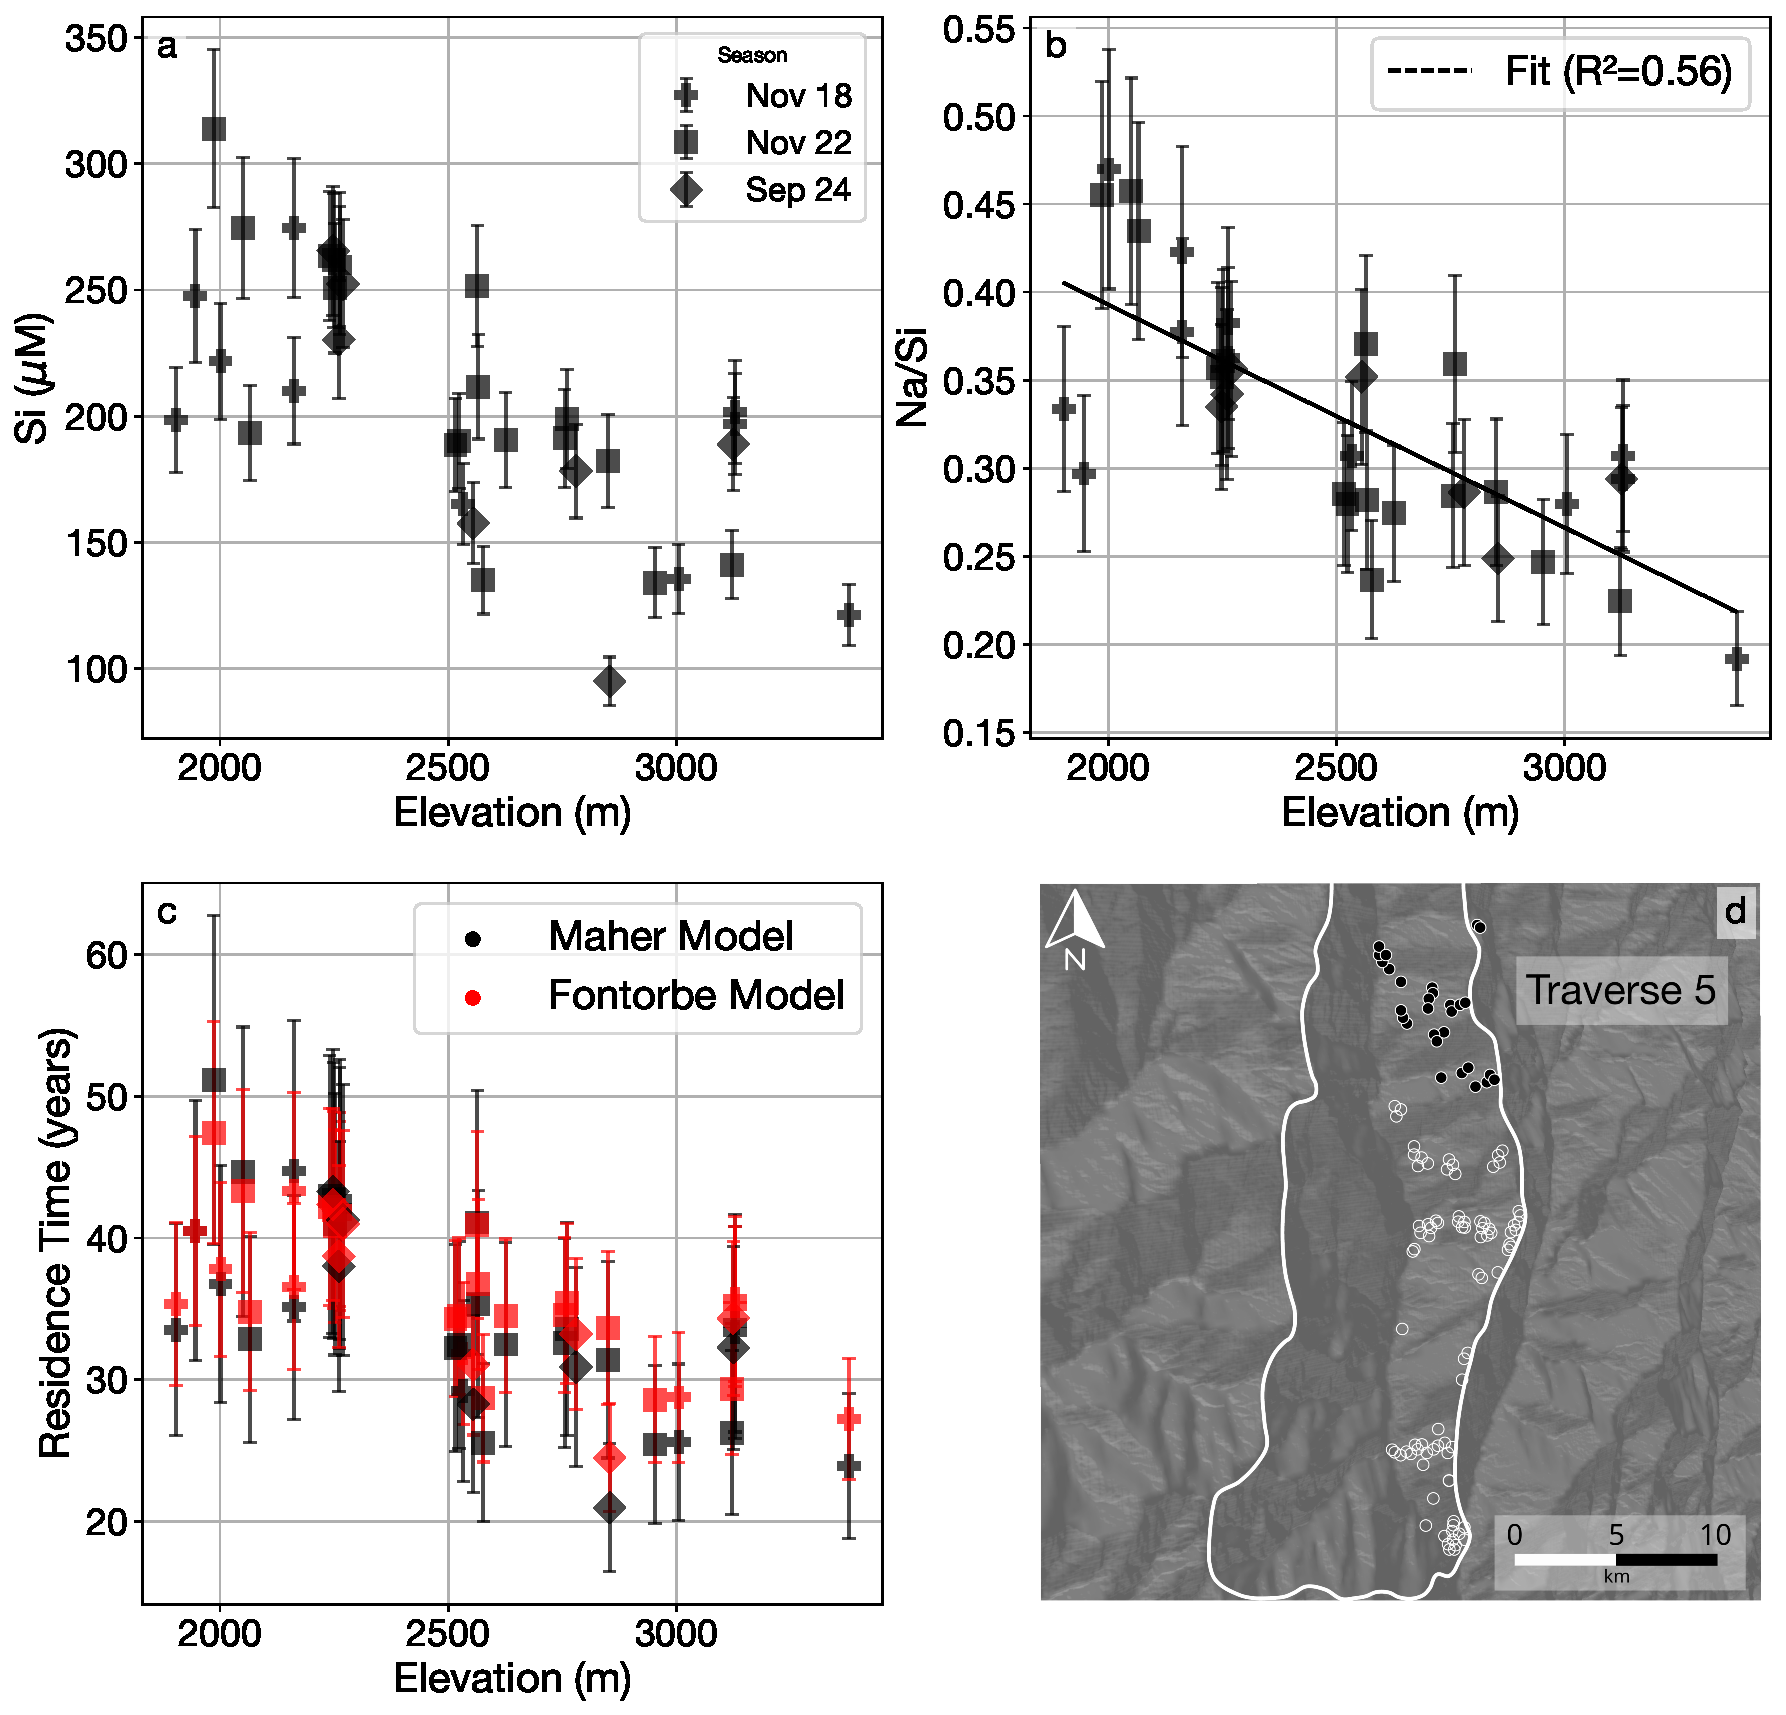
\includegraphics[width=\textwidth]{Traverse_5_summary.pdf}
    \caption{Traverse 5 - Variations in Spatial Chemistry}
    \label{fig:spatial_changes_spring5}
\end{figure}

\FloatBarrier

Traverse 5 is highly sampled and sits at the highest elevation of the whole catchment. DSi concentration increases with decreasing elevation but there is noticeable scatter in the data. Na/Si similarly shows a trend of increasing ratio with decreasing elevation, and it is replicated between different seasons, with considerable scatter. Residence times are the lowest predicted in the catchments, and so are the strontium isotope values.


\subsection{Time Series Trends}

Concentrations of dissolved silicon in several springs in the catchment show a consistent decrease in concentration with the onset of the monsoon. Concentrations are high in April, decrease to a minimum in September, then slowly increase back to April levels through October and November. Decrease in concentration is likely a sign of dilution from increased precipitation during the monsoon. Such a trend is also present in a time series of a spring in Traverse 3. The average April-September decrease is small compared to the average dissolved silicon concentration of the rain.


\begin{figure}[h]
    \centering
    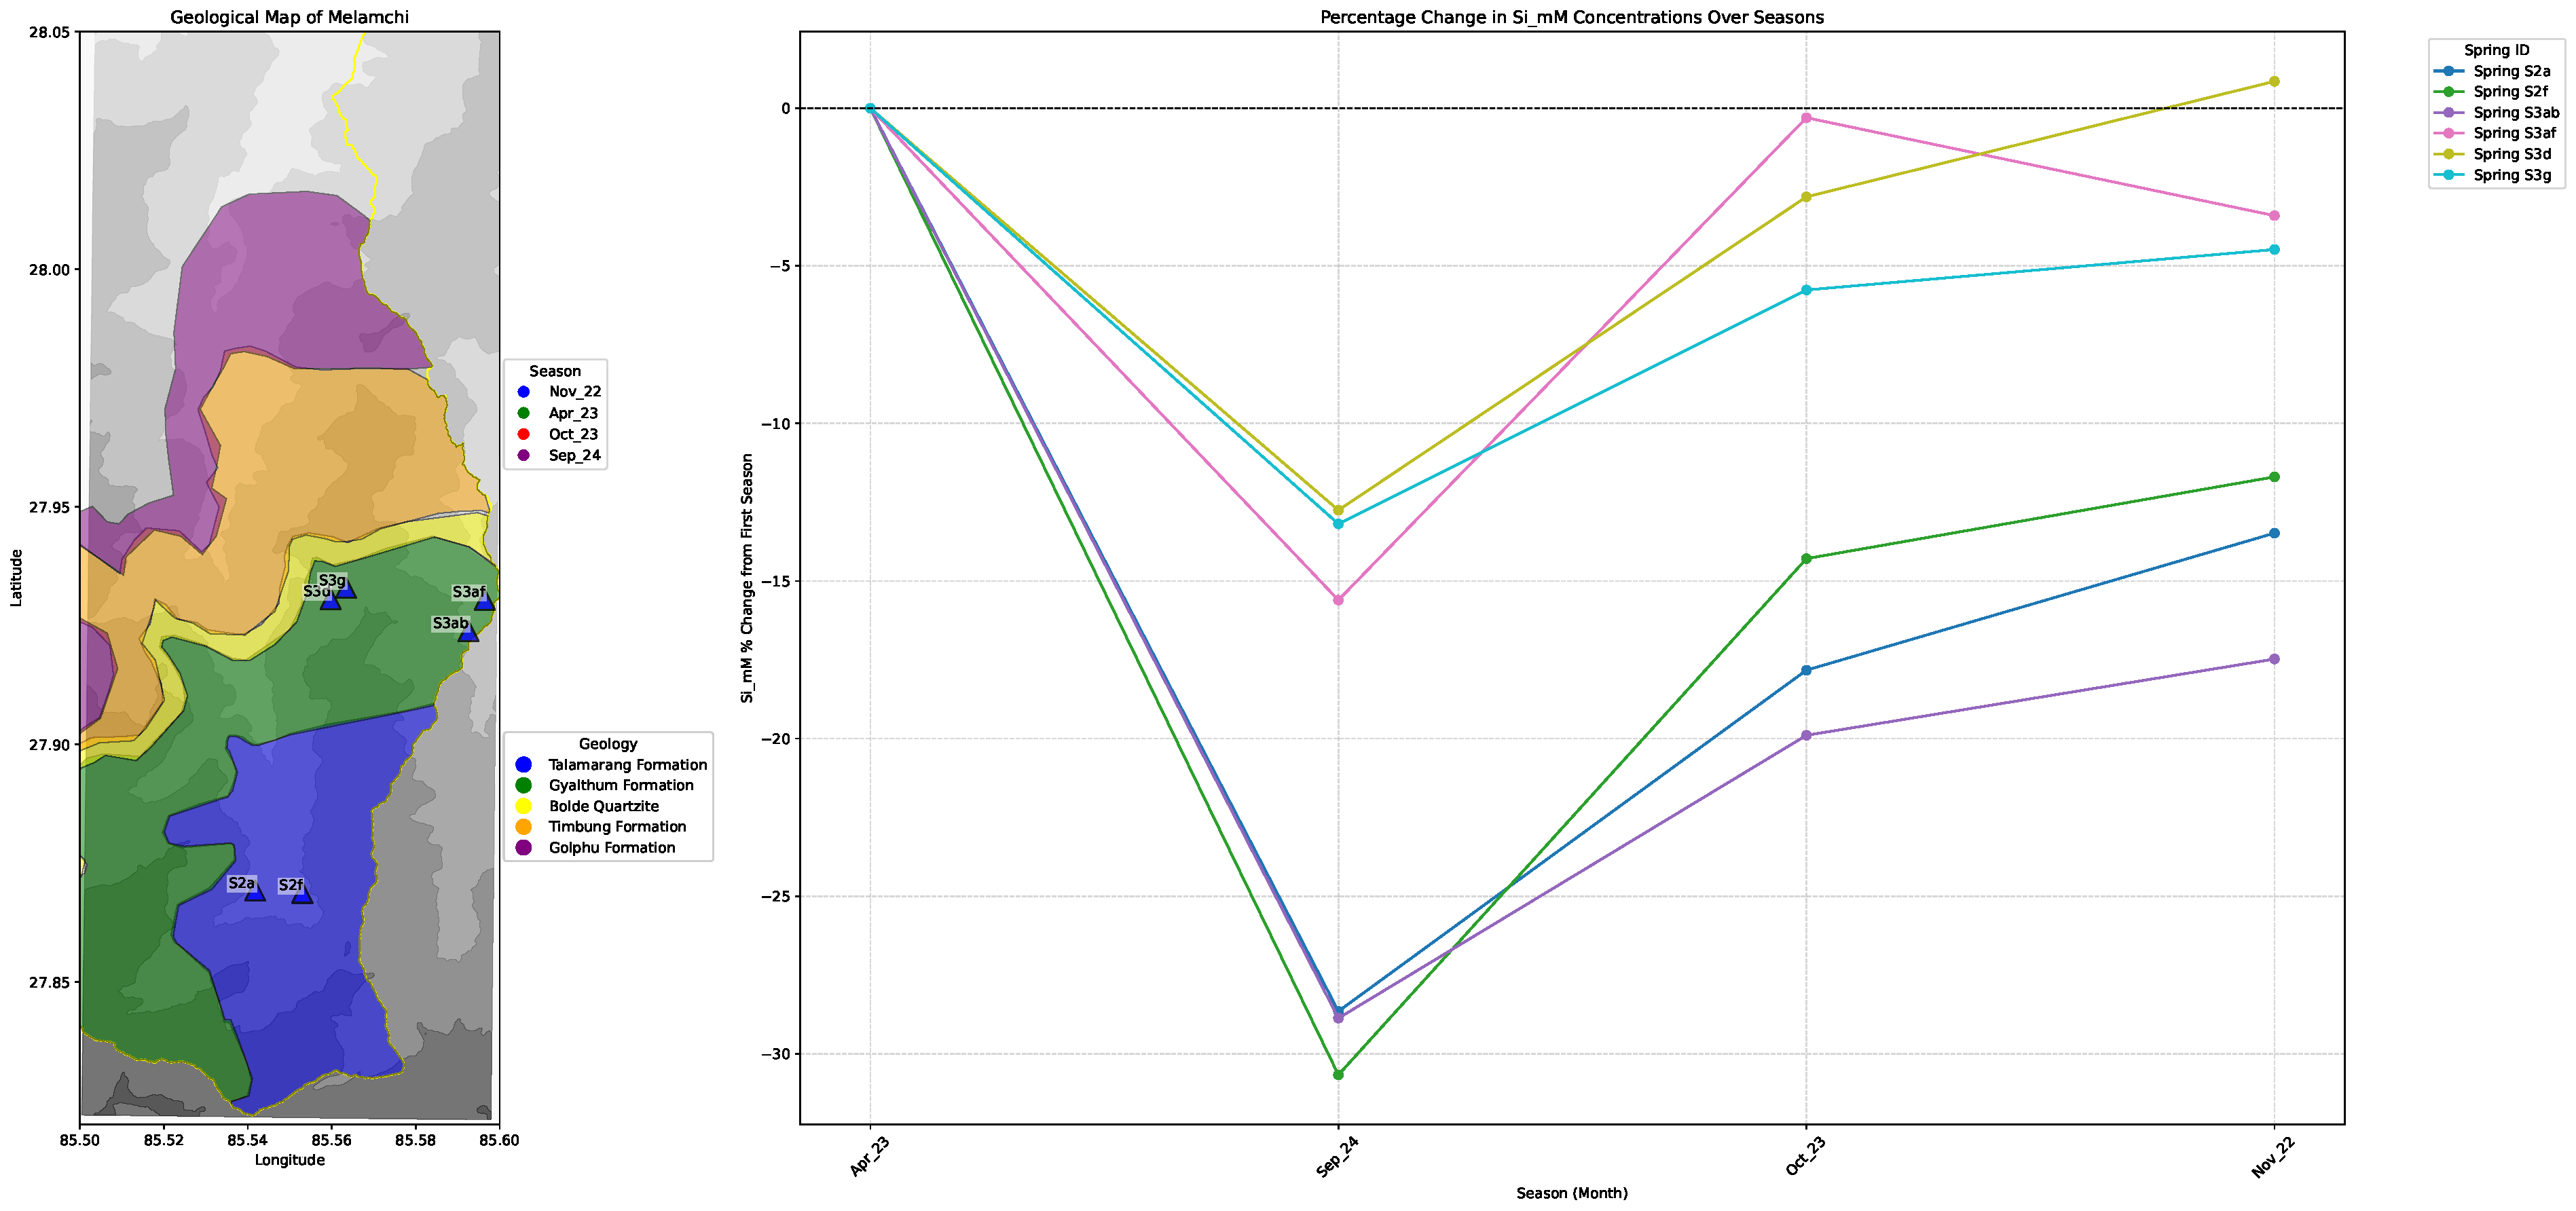
\includegraphics[width=0.8\textwidth]{Si_mM_percentage_change_springs.pdf}
    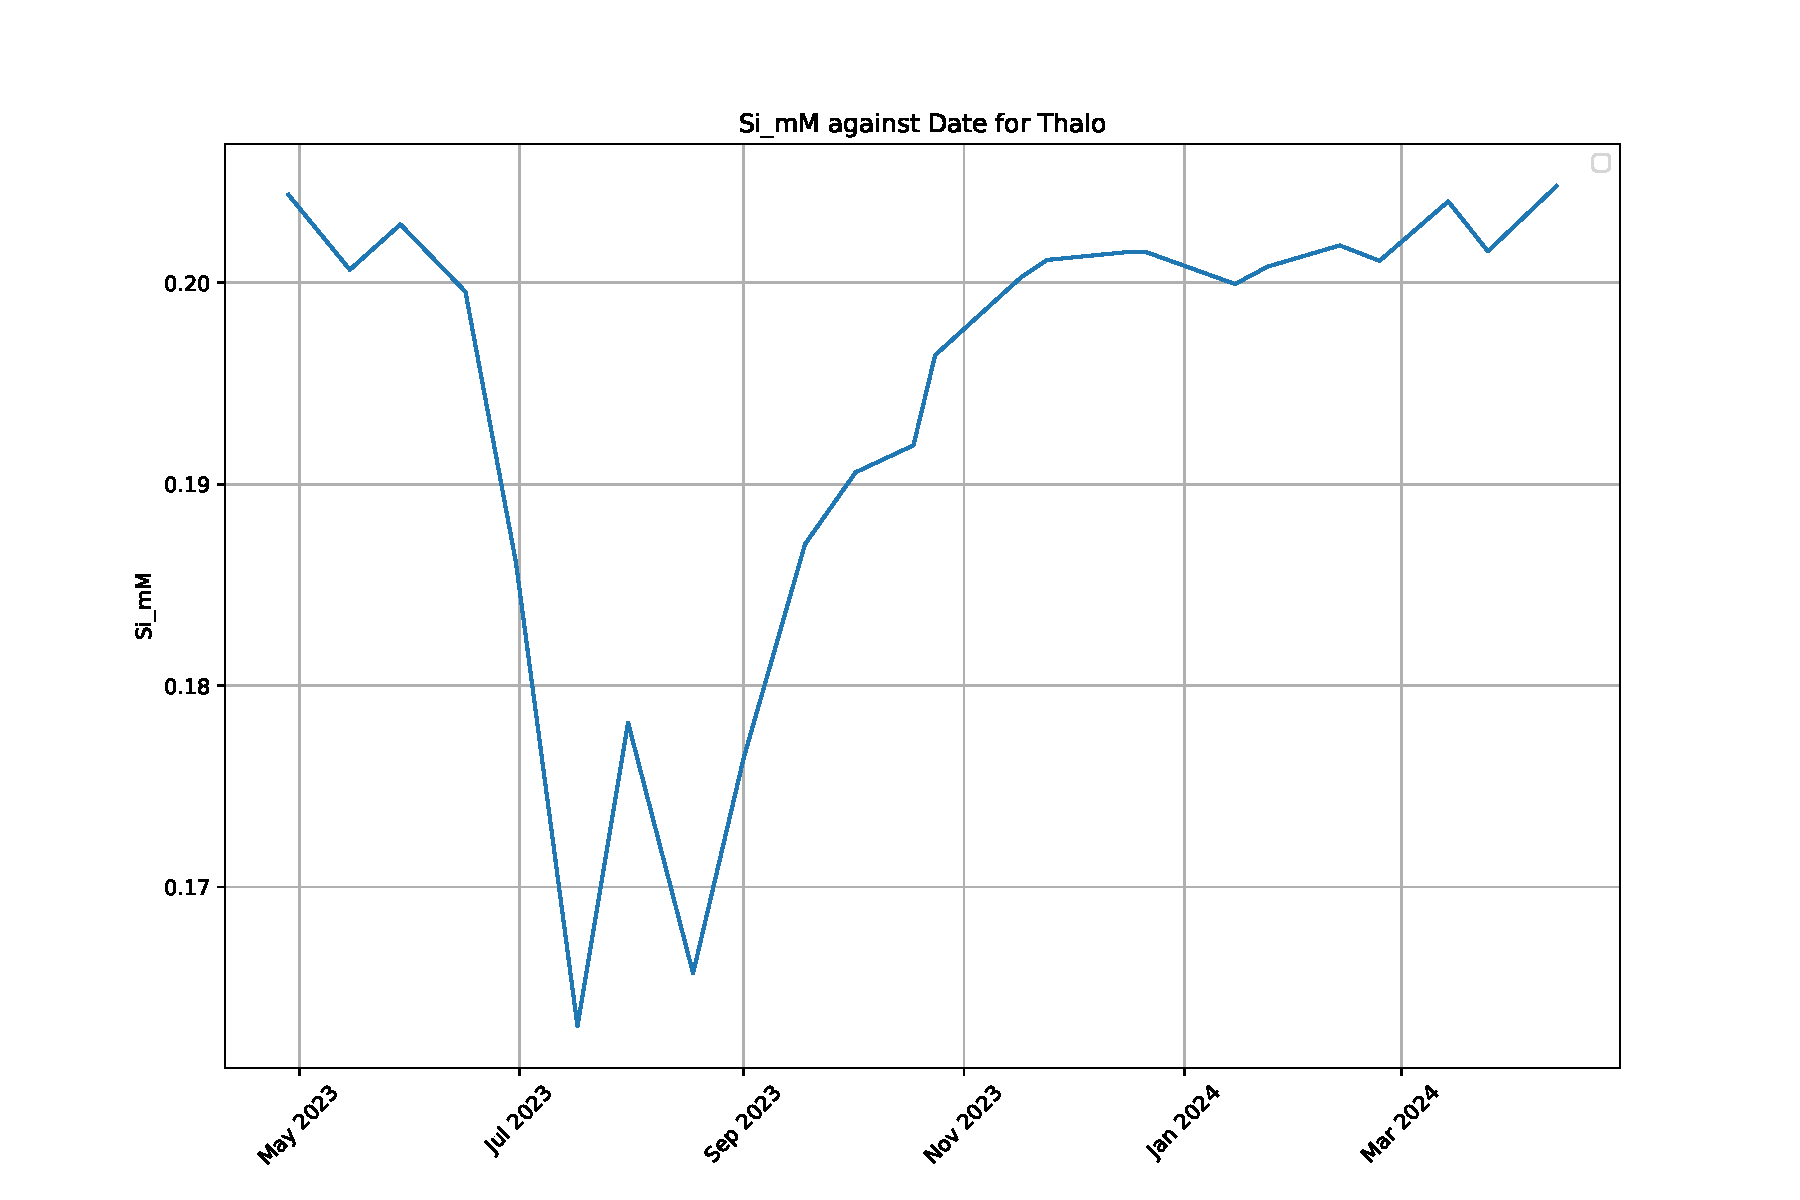
\includegraphics[width=0.8\textwidth]{Si_mM_Thalo_timeseries.pdf}
    \caption{Seasonal changes in spring concentration indicating monsoonal precipitation influence.; Time series of spring concentration changes over time.}
    \label{fig:time_series_changes}
\end{figure}

\FloatBarrier
